\section{Elaboration Time Hardware Construction}
\label{sec:elab}
The methods for constructing hardware in the previous chapters are all
similar in that the user directly interfaces with them. The user
directly constructs the directed subgraph of {\tt Nodes} that
implements the desired circuit and connects that subgraph to the main
graph. We refer to that class of hardware construction as 
{\it runtime} hardware construction since the hardware is
constructed as Scala is making a pass over user-written code. This
chapter discusses another class of hardware construction that we refer
to as {\it elaboration time} hardware construction since the
hardware is constructed during Chisel elaboration. This class of
hardware construction is useful since it is not always possible or
desirable for the user to construct the circuit as they are building
up the Chisel graph. The remainder of this chapter presents the
interface for writing elaboration time hardware construction routines
and three examples of how to use that interface.

\subsection{Elaboration Time Hardware Construction Interface}
The Chisel compiler maintains a list of functions that it invokes
during elaboration time to refine the input user graph of 
{\tt Nodes}. These functions must adhere to the interface described in
Figure~\ref{fig:transforms}. The bodies of the functions in
Figure~\ref{fig:transform1} varies from transformation to
transformation but will usually follow two phase format. The first
phase performs some analysis on the Chisel graph to collect
information, e.g. find all Reg nodes. The second phase will then use
the information from the first phase to construct a circuit and
perform some transformation on the graph, e.g. generate an enable
circuit for every Reg node and connect the circuit into the Reg node.

\begin{figure}[htb]
\centering
  \begin{subfigure}[t]{0.48\textwidth}
  \centering
  \caption{Elaboration Time Functions}
  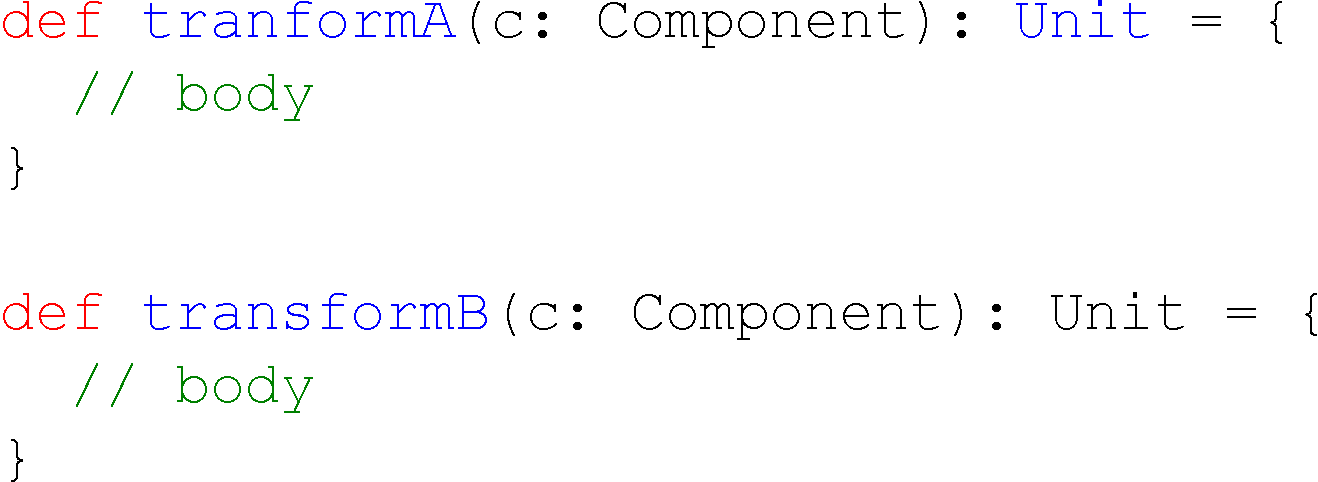
\includegraphics[width=0.9\textwidth]{figures/transform1.pdf}
  \label{fig:transform1}
  \end{subfigure}
  \hfill
  \begin{subfigure}[t]{0.48\textwidth}
  \centering
  \caption{Elaboration Time Hook}
  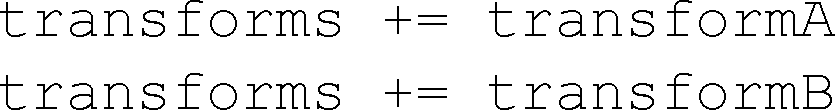
\includegraphics[width=0.7\textwidth]{figures/transform2.pdf}
  \label{fig:transform2}
  \end{subfigure}
\caption{Elaboration Time Interface}
\label{fig:transforms}
\end{figure}

\subsection{When}
Chisel provides a {\tt when - elsewhen - otherwise} statement for
performing conditional updates on {\tt Bits} and {\tt Reg}
nodes. This statement appears behavioral but actually constructs a
hardware circuit to perform the update. The construction of this
circuit is delayed until elaboration time since it is easier to
construct the circuit once the user has specified all the updates than
it is to construct the circuit as the user is specifying
updates. 

\begin{figure}[htb]
\centering
  \begin{subfigure}[t]{0.48\textwidth}
  \centering
  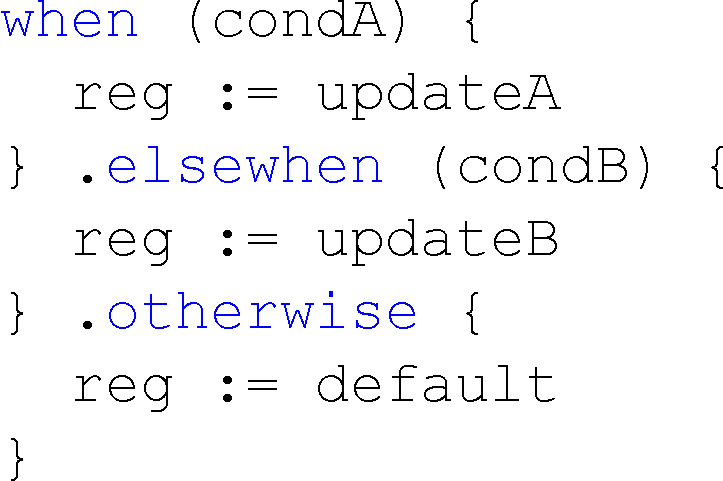
\includegraphics[width=0.7\textwidth]{figures/when.pdf}
  \caption{When Code}
  \label{fig:whenscala}
  \end{subfigure}
  \hfill
  \begin{subfigure}[t]{0.48\textwidth}
  \centering
  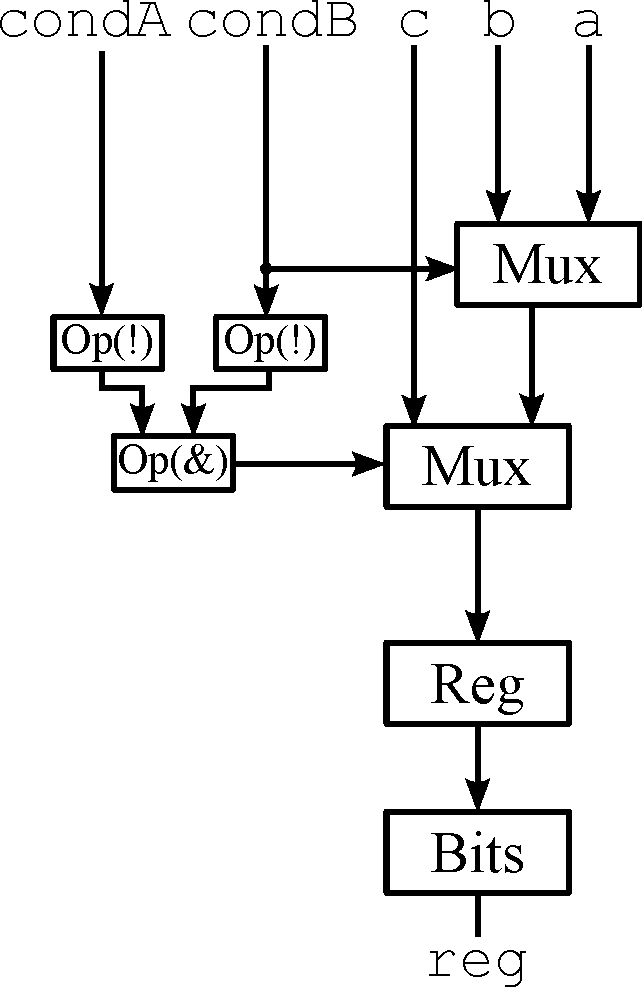
\includegraphics[width=0.5\textwidth]{figures/whengraph.pdf}
  \caption{When Graph}
  \label{fig:whenelab}
  \end{subfigure}
\caption{When Statement}
\label{fig:when}
\end{figure}

{\bf Runtime}. Instead of constructing hardware whenever a {\tt when}
statement is executed, we simply record information to be used during
elaboration. For this purpose, we maintain a mapping of node to list
of update tuples with the format {\tt (cond, bits)} where {\tt cond}
is the condition of the when statement and {\tt bits} is the update
data. These update tuples are constructed for every update statement
within the body of a {\tt when} statement and appended to the list
mapped to the node on the left hand side of that update
statement. Note that the updates in this list do not have to be
mutually exclusive. In the case when multiple updates are enabled,
Chisel has the semantics that the last update in program order (i.e
the last update in the list of updates) takes priority.

Figure~\ref{fig:whenscala} shows an example usage of when statements
to conditionally update a register. When this statement is executed,
it will add 3 update tuples to {\tt reg}'s list of update tuples. The
first statement adds the tuple {\tt (condA, updateA)}, the second adds
{\tt (condB \&\& !condA, updateB)}, and the third adds
{\tt (!condB \&\& !condA, updateC)}.

{\bf Elaboration Time}. The elaboration time transformation function
does not need to perform any analysis since we store all the
information for elaboration during runtime in the form of a mapping
from node to list of update tuples. For each entry in this mapping, we
construct a chain of {\tt Mux} nodes from the list of update tuples and
connect the output of that chain into the input of the node in the
mapping. If the node in the mapping is a {\tt Reg} node then nothing
is done for the case when no updates are enabled. Otherwise, the node
in the mapping is a {\tt Bits} node and we have an additional {\tt Mux}
node to mux out a default signal provided by the user. If no default
signal is provided, Chisel reports an error to the user.

\subsection{SRAM Backend}
Users targeting the Verilog backend will want to map Mems to SRAMs
with backend specific SRAM interfaces. One way to target these SRAM
interfaces is to encode the interface into the Chisel user code. This
has the disadvantageous effect of muddling the code with SRAM specific
information and makes it an unnecessarily tedious to compile the Chisel
for a different SRAM backend.

A better way to target backend specific SRAM interfaces is to write an
elaboration time function that transforms the Chisel graph to target
specific SRAM interfaces. Let's say we want to target an SRAM that has
an {\tt init} pin which needs to be wired to the top level module. We
first perform either a breadth first search or depth first search to
find all {\tt Mem} nodes in the graph. For every {\tt Mem} node, we
create a new {\tt Bits} node to stand in for the {\tt init} pin. We
add this node to the {\tt Mem} node's input. Finally, we walk up the
{\tt Component} hierarchy starting at the {\tt Component} that
contains the {\tt Mem} node and ending at the top level
{\tt Component}. For every {\tt Component} along this path, we create
a new port to connect up the {\tt init} pin.

Targeting SRAM interfaces in this way allows us to decouple the
SRAM backend from the user code. If we want to switch to a different
SRAM target we only need to switch to a different elaboration time
function and do not need to modify the user code.

\subsection{Automatic Pipeline Synthesis}
\begin{figure}[htb]
\centering
  \begin{subfigure}[t]{0.8\textwidth}
  \centering
  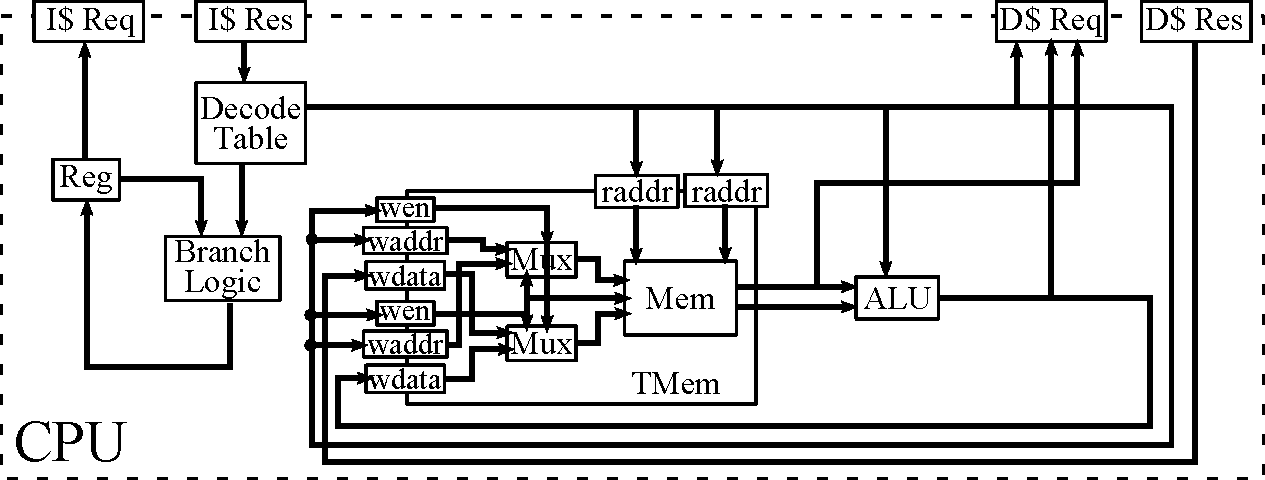
\includegraphics[width=\textwidth]{figures/pipeline.pdf}
  \caption{{\bf Datapath Graph}. CPU datapath represented as a
    directed dataflow graph in Chisel.}
  \label{fig:datapathgrah}
  \end{subfigure}
  \begin{subfigure}[t]{0.8\textwidth}
  \vspace{20pt}
  \centering
  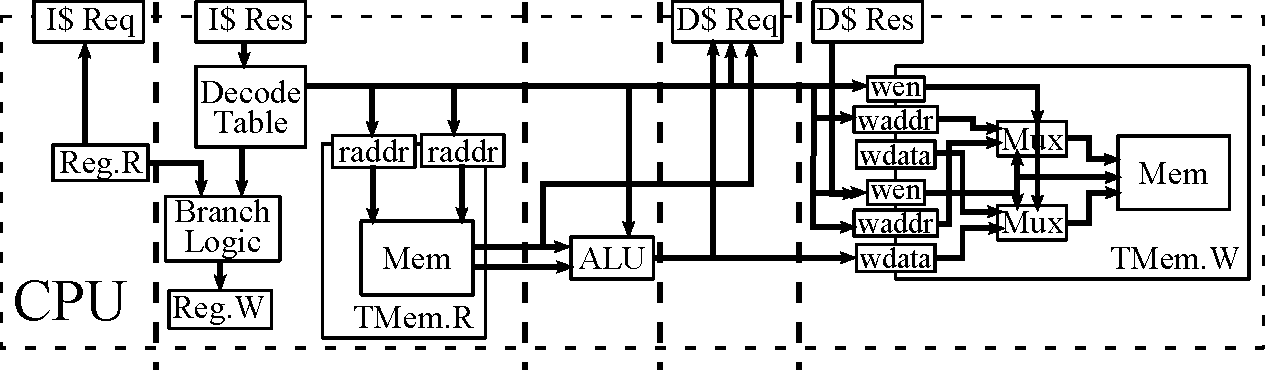
\includegraphics[width=\textwidth]{figures/pipelinedag.pdf}
  \caption{{\bf Datapath DAG}. 5-stage CPU datapath turned into a
    directed acyclic graph by breaking {\tt Reg} nodes and {\tt
      TransactionalMem} into read and write ports. The dashed lines
    represent pipeline boundaries.}
  \label{fig:datapathdag}
  \end{subfigure}
\caption[5-stage CPU Datapath]{{\bf 5-stage CPU Datapath}. ALU = arithmetic logic unit. D\$
  = data cache. I\$ =  instruction cache. TMem =
  TransactionalMem. {\tt x}.R = read port of node {\tt x}. {\tt x}.W =
  write port of node {\tt x}}
\label{fig:datapath}
\end{figure}

Pipelining is a commonly used microarchitectural technique for
improving the performance of a datapath. Hardware designers usually
determine up front the desired pipeline depth and then bake the
corresponding pipelining logic into their datapath code. This approach
clutters an otherwise easy to read datapath with extraneous logic
unrelated to original functionality of the datapath, making it
difficult to modify the datapath or even change the pipeline depth. A
better approach that overcomes these issues is to separate the
pipelining logic from the datapath specification~\cite{hoe:syn}. The
designer provides only the datapath and pipeline specification. Then during
elaboration, Chisel generates the pipelining logic.

{\bf Datapath and Pipeline Specification}. In our approach, the Chisel
datapath code that implements a transaction is maintained separate of
the datapath's pipeline specification. The datapath code is viewed as
a set of architectural state elements and next-state logic that reads
the architectural state and computes the updates. We use {\tt Reg}
nodes and {\tt TransactionalMem}s to represent architectural
state. For {\tt Reg} nodes, we view the enable signal and the
update signal as the {\tt wen} and {\tt wdata} of the Reg. The {\tt Reg}
node itself is treated as the {\tt rdata}. A {\tt TransactionalMem} is
a Chisel {\tt Component} that wraps a Chisel {\tt Mem} node. 
{\tt TransactionalMem}s are instantiated with the desired number of
{\it virtual} write ports and {\it physical} write ports. Each
virtual write port has an explicit {\tt wen}, {\tt wdata}, and {\tt waddr}
port. The {\tt TransactionalMem} generates the logic to multiplex the
virtual write ports over the physical write ports if there are more
virtual write ports than physical write ports.

Our pipeline synthesis tools provides the functions
{\tt setPipelineComponent} for specifying the datapath to pipeline,
and {\tt setPipelineStage } for specifying in what pipeline stage a {\tt Node}
or {\tt Component} belongs. These functions allow the user to
succinctly describe a pipeline and unclutter the datapath code since
the pipeline specification can be maintained independent of the datapath.

{\bf Pipeline Generation}. During elaboration our pipeline synthesis
tool reads the datapath and pipeline specification to determine
register placement. We first mark nodes with the stage number that the
user has indicated in their pipeline specification. For each node with
a stage number we propagate the node's stage numbers to node's
producers and consumers in a breadth first search like manner. We only
propagate a stage number if (1) the node currently does not have a stage
number conflict and (2) all of its children (producer and consumer nodes)
are ready to receive a stage number. When receiving a stage number, a
node will take a stage number that is either equal to the max stage number of
its producers (if the node is receiving a propagation from its producer
side) or equal to the min stage number of its consumers (if the node is
receiving propagation from its consumer side).

Nodes can be marked with multiple stage numbers since it is possible to
reach nodes from different pipeline stages. Our tool adds pipeline
registers to the node's inputs (between the node and its producer) or
to the node's outputs (between the node and its consumer) to resolve
stage number conflicts. Resolving a node's stage number conflict
before propagation allows our tool to more deterministically assign
stage numbers.

A node is ready for propagation from the producer side if all of its
producers have a stage number. Likewise, a node is ready for
propagation from the consumer side if all of its consumers have a
stage number.

Once all nodes are marked with a stage number, we make one final pass
through the Chisel graph to insert pipeline registers between adjacent
nodes with different stage numbers.

\begin{figure}[htb]
\centering
  \begin{subfigure}[t]{0.8\textwidth}
  \centering
  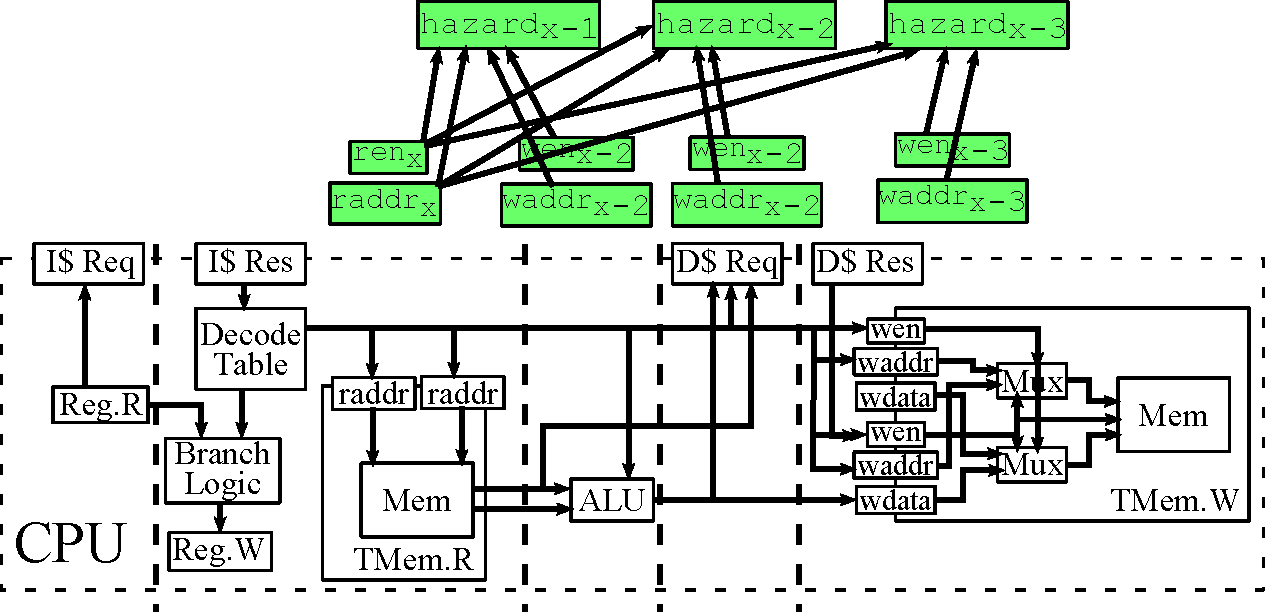
\includegraphics[width=\textwidth]{figures/pipelinehazard.pdf}
  \caption{{\bf Hazard Detection}. All the hazards that
    the {\tt TransactionalMem} generates in a 5-stage pipeline.}
  \label{fig:haz}
  \end{subfigure}
  \begin{subfigure}[t]{0.8\textwidth}
  \vspace{20pt}
  \centering
  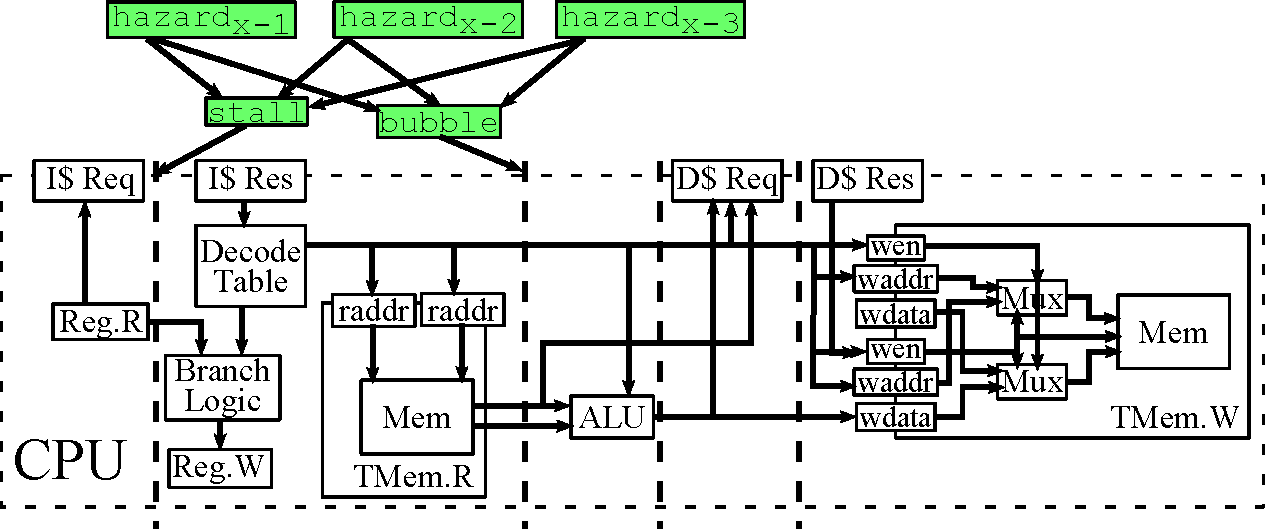
\includegraphics[width=\textwidth]{figures/pipelineinterlock.pdf}
  \caption{{\bf Interlocks}. The hazard conditions stall the
  first and second stage and push bubbles into the third stage.}
  \label{fig:int}
  \end{subfigure}
\caption{Resolving hazards through interlocks}
\label{fig:hazint}
\end{figure}

{\bf Hazard Detection}. Inserting pipeline registers into the datapath
graph introduces pipelining hazards that are not present in the
unpipelined datapath. Here we discuss how to handle data hazards which
result from a transaction reading a state element (a {\tt Reg} node or a
{\tt TransactionalMem}) before an earlier transaction writes to that state
element. 

We first search through the datapath graph to find all state
elements. For every state element, we determine whether or not a
hazard exists on it. If there is a hazard on a state element, we add
the hazard condition into a list. For {\tt Reg} or {\tt TransactionalMem}, a
hazard condition exists if the state element belongs in a stage that precedes the
stage of its write enable or write data signal. The actual Boolean
hazard condition is {\tt wen \&\& ren} for a {\tt Reg} node and
{\tt wen \&\& ren \&\& waddr == raddr} for a {\tt TransactionalMem}.

Figure~\ref{fig:haz} shows the hazard conditions that our tool
identifies on the {\tt TransactionalMem}. when analyzing the generated pipeline in
Figure~\ref{fig:datapathdag}. We first search the pipeline for all
state elements. In this example, the {\tt Reg} node and the 
{\tt TransactionalMem} are the only state elements. We then examine
the read and write ports of these state elements to determine whether
or not there are any hazards. The {\tt Reg} has its write port in the
second stage but its read port is in the first stage. So we generate a
hazard signal in the first stage. The {\tt TransactionalMem} has its
write port in the fifth stage but its read port is in the second
stage. We trace backwards from the {\tt wen} in the fifth stage to the
second stage to find all the other {\tt wen} signals. For each 
({\tt wen}$_i$, {\tt waddr}$_i$) pair, we generate a hazard condition
{\tt wen$_i$ === ren$_i$ \&\& waddr$_i$ === raddr}.

{\bf Hazard Resolution - Interlocks}. The easiest way to resolve
hazards is through interlocks. This hazard resolution method requires
no additional input from the user. Every identified hazard is placed
into the stage of the read port that generates the hazard. In
Figure~\ref{fig:haz}, the hazards would be placed into the second
stage because the corresponding read port is in the second stage. We
then go through every stage and perform an {\tt OR} reduction on all
the hazards in that stage as well as all the hazard conditions in the
following stages to produce the stall condition for that stage. The
second part of interlocking a pipeline is to push bubbles. We go
through every stage and generate a {\tt pushBubble} signal if there is
a hazard condition in that stage and no following stages have a
hazard.

Figure~\ref{fig:int} shows the interlock logic that our tool
generates to handle the hazards from Figure~\ref{fig:haz}. Since
the {\tt TransactionalMem}'s read port is in the second stage, all the
{\tt hazard$_i$}s go into the second stage. When examining the second
stage, the tool would {\tt OR} reduce all the {\tt hazard}$_i$s to
generate a stall condition in the second stage. This stall condition
is used to stall the second and first stage. The same hazard
condition is then used to generate the {\tt pushBubble} signal. There
are no other sources of hazards further down the pipeline so the
hazard condition in the second stage is sufficient for pushing a
bubble into the second stage. Although not shown, we also generate
interlock logic for {\tt Reg} whose read port is in stage one and
write port is in stage two. We generate a hazard condition in the
first stage that is used to stall only the first stage. A bubble is
pushed into stage two if this hazard condition is asserted the second
stage's hazard condition is not asserted.

\begin{figure}[htb]
\centering
  \begin{subfigure}[t]{0.8\textwidth}
  \centering
  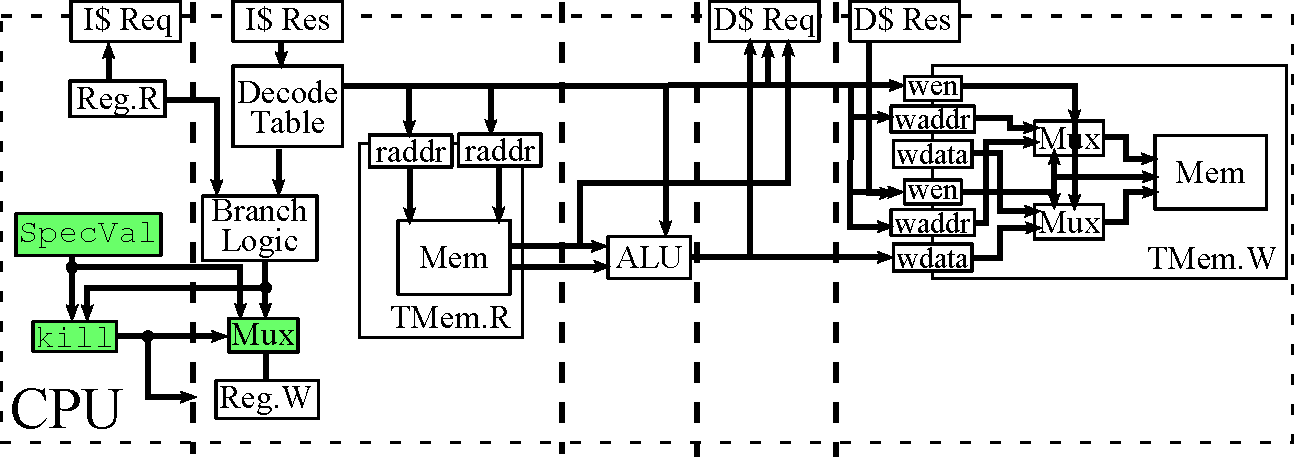
\includegraphics[width=\textwidth]{figures/pipelinespec.pdf}
  \caption{{\bf Speculation}. Using speculation to resolve hazards on
    the {\tt Reg} node whose read port is in the first stage and write port
  is in the second stage.}
  \label{fig:spec}
  \end{subfigure}
  \begin{subfigure}[t]{0.8\textwidth}
  \vspace{20pt}
  \centering
  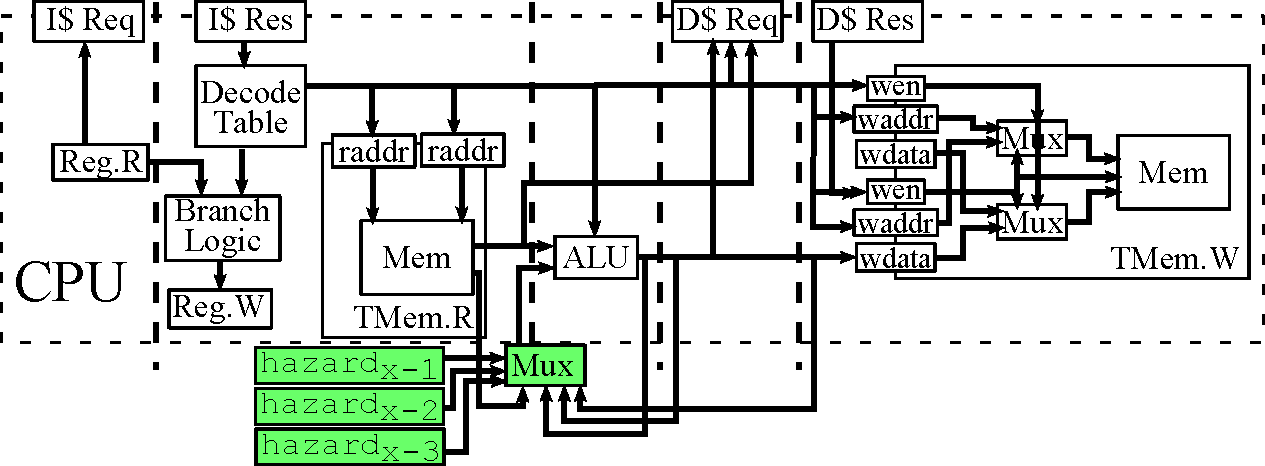
\includegraphics[width=\textwidth]{figures/pipelinebypass.pdf}
  \caption{{\bf Bypassing}. Bypassing network generated to forward ALU
  results from the third stage, fourth stage, and fifth stage to the
  {\tt TransactionalMem}'s second read port.}
  \label{fig:bypass}
  \end{subfigure}
\caption{Resolving hazards through speculation and bypassing}
\label{fig:specbyp}
\end{figure}

{\bf Hazard Resolution - Speculation}. Our tool provides the function
{\tt speculate} that users can use to specify the stage element whose
write value they want 
to speculate along with the value they want to use for
speculation. This hazard resolution option is useful for transactions
that produce data that takes on one value with a very high likelihood
since we can have dependent transactions guess that value, allowing us
to avoid stalls. In a processor pipeline, for example, transactions
will usually write {\tt PC+4} to the PC register. To take advantage of
this regularity, we can guess that every transaction will write {\tt
  PC+4} to the {\tt PC} register. During elaboration, we modify the
Chisel graph to use the speculation value that the user provides to
update the node that the user marks for speculation. The speculation
value is pipelined until the actual data value is produced. We compare
the speculation value to the actual value. If the values match, we
continue as normal. Otherwise, we flush every stage starting at the
speculation stage up to but not including the stage where the
speculation value is checked.

To see how our speculation tool works, let's examine the pipeline in
Figure~\ref{fig:spec}. Notice that since every
transaction writes to the {\tt Reg} node in the second stage while
another transaction reads the node in the first stage, the interlock
hazard resolution option would cause our pipeline to stall every other
cycle. This scenario is a good match for the speculation resolution
option since transactions tend to write a very predictable value into
that node. We use the {\tt speculate} function to indicate that we
are guessing that the {\tt Reg} node will take on {\tt SpecVal}. We
mux in {\tt SpecVal} into the {\tt Reg} and then pipeline {\tt
  SpecVal} once (since the {\tt Reg} is read in the first stage and
written in the second stage). We compare {\tt SpecVal} to the actual
value to generate a kill signal that is asserted whenever the two
signals do not match. The kill signal is used to write the correct
value into the {\tt Reg} and we kill stage one.

{\bf Hazard Resolution - Bypassing}. Transactions that depend on the
results of previous transactions can make use of bypass networks to
receive these results instead of interlocking until those results are
committed. Our tool provides the functions {\tt bypassTo} to annotate
a read port for bypassing and {\tt avoidBypassFrom} to annotate that a
write path should not be bypassed. During elaboration, the pipeline
synthesis tool generates the appropriate bypassing network. For each
read port, the tool traces backwards from the corresponding write port
to find all {\tt wen}, {\tt wdata}, and {\tt waddr} signals and filters
out the write ports from {\tt avoidBypassFrom}. For each ({\tt wen},
{\tt wdata}, {\tt waddr}) tuple that the tool finds, generate a mux
at the read port to mux out {\tt wdata} whenever {\tt wen \&\& waddr
  === raddr} giving priority to ({\tt wen}, {\tt wdata}, {\tt waddr})
tuples from earlier pipeline stages. We then search for that condition
in the hazard list and remove it to avoid generating the interlock
logic for that condition. 

Figure~\ref{fig:bypass} shows an example bypass network. In this
example, the user annotates the second read port of the {\tt
  TransactionalMem} with {\tt bypassTo} function and has told the tool
to not bypass from the data cache with the {\tt avoidBypassFrom}
function. The tool generates a chain of three muxes since it found three
write paths out of the ALU in the third, fourth, and fifth stage.
